\documentclass{beamer}


\usepackage{amsmath}
\usepackage[style=alphabetic,url=true]{biblatex}
\usepackage{environ}
\usepackage{geometry}
\usepackage{graphicx}
\usepackage{tikz}
\usepackage[T2A]{fontenc}
\usepackage[utf8]{inputenc}
\usepackage[cache=false]{minted}
\usepackage{amsmath}
\usepackage{amsfonts}
\usepackage{amssymb}
\usepackage{calrsfs}


% \usetheme{Bergen}

\usecolortheme{beaver}

\setbeamertemplate{itemize item}[circle]
\setbeamertemplate{itemize subitem}{--}
\addtobeamertemplate{navigation symbols}{}{
  \usebeamerfont{footline}%
  \usebeamercolor[fg]{footline}%
  \hspace{1em}%
  \insertframenumber/\inserttotalframenumber
}
\graphicspath{ {./graphics/} }
\setminted[Python]{
  fontsize=\tiny
}
\BeforeBeginEnvironment{minted}{\medskip}
\AfterEndEnvironment{minted}{\medskip}



\title{
  Bitcoin and Cryptocurrency Technologies \\
  Lecture 4: Bitcoin Data Model
}

\author{Yuri Zhykin}
\date{Apr 27, 2022}

\begin{document}

\frame{\titlepage}

\begin{frame}
  \frametitle{Bitcoin Data Model}
  \begin{itemize}
  \item \textbf{Bitcoin Block Chain} (or \textbf{Bitcoin Time Chain} is a
    distributed, highly-redundant database of transaction records that strongly
    guarantees the \textit{existence, validity and order} of transactions.
  \item \textbf{Bitcoin Protocol} is a distributed protocol of maintaining the
    Bitcoin transaction database that imposes strict rules about transaction
    validity and enforces the database guarantees through the
    \textbf{Proof-of-Work} system.
  \item If a transaction record is added to the database, one can be sure that
    it 
    \begin{itemize}
    \item definitely happened,
    \item is provably valid,
    \item it happened strictly before or after the other transactions.
    \end{itemize}
  \end{itemize}
\end{frame}

\begin{frame}
  \frametitle{Transaction}
  \begin{itemize}
  \item \textbf{Tx}
    \begin{itemize}
    \item \textbf{version}
    \item \textbf{inputs}
    \item \textbf{outputs}
    \item \textbf{witnesses}
    \item \textbf{locktime}
    \end{itemize}
  \item \textbf{Inputs} - a list of transaction inputs - references to the
    outputs of other transactions, that are consumed by this transaction.
  \item \textbf{Outputs} - a list of newly created outputs that specify, where
    all the bitcoin from the outputs referenced by inputs is being transferred.
  \item \textbf{Locktime} restricts the moment in time, when the transaction can
    be included in the transaction records database.
  \end{itemize}
\end{frame}

\begin{frame}[fragile]
  \frametitle{Transaction ID}
  \begin{itemize}
  \item \textbf{Transaction ID} is not included in the transaction data
    structure, since it can be computed from the binary representation of the
    transaction:
    $$TXID = SHA256(SHA256(TX_{binary})$$
  \item $TXID$ is a 32-byte sequence and is usually represented as a
    64-character hex-encoding of the 32-byte sequence:
    \begin{minted}{Python}
      169e1e83e930853391bc6f35f605c6754cfead57cf8387639d3b4096c54f18f4
    \end{minted}
  \end{itemize}
\end{frame}

\begin{frame}
  \frametitle{Transaction Output}
  \begin{itemize}
  \item \textbf{TxOutput}
    \begin{itemize}
    \item \textbf{amount}
    \item \textbf{lock-script}
    \end{itemize}
  \item \textbf{Amount} - an amount of bitcoin currency units, called
    ``satoshis'' represented as an integer (1 BTC = $10^8$ satoshis).
  \item \textbf{Lock-script} - a computational (usually ``supply a valid
    signature'') problem that must be solved in order to spend this output,
    expressed as Bitcoin Script program.
  \end{itemize}
\end{frame}

\begin{frame}
  \frametitle{Transaction Input}
  \begin{itemize}
  \item \textbf{TxInput}
    \begin{itemize}
    \item \textbf{previous-tx-id}
    \item \textbf{previous-tx-index}
    \item \textbf{unlock-script}
    \end{itemize}
  \item Transaction input is a reference to the transaction output being spent
    along with the solution to the lock-script of that output.
  \item \textbf{Previous transaction ID} - a TXID of the transaction that
    created the output.
  \item \textbf{Previous transaction index} (\textbf{VOUT}) - an index of the
    output in the output list of the transaction referenced by previous
    transaction ID.
  \item \textbf{Unlock-script} - a solution to the \textit{lock-script} of the
    output being spent represented as Bitcoin Script program.
  \end{itemize}
\end{frame}

\begin{frame}
  \frametitle{Transaction Witness}
  \begin{itemize}
  \item \textbf{Witness} is an additional structure in the transaction that was
    introduced as a protocol upgrade (called \textbf{SegWit} -
    \textbf{Seg}regated \textbf{Wit}ness) in 2017 as a first step in a long-term
    plan to improve Bitcoin security, scalability and flexibility.
  \item \textbf{Witness} allows to store complex \textit{unlock-scripts}
    (solutions) to the \textit{lock-scripts}, which accounts for a large part of
    the transaction size.
  \end{itemize}
\end{frame}

\begin{frame}
  \frametitle{UTXO (Unspent Transaction Output) Set}
  \begin{itemize}
  \item All bitcoin in existence is represented via a set of \textbf{unspent
      transaction outputs} (\textbf{UTXOs}) - a set of records of the form
    $(amount, owner)$ that can be provably verified as not used in any
    known transaction.
  \item Every regular Bitcoin transaction consumes some existing UTXOs and
    generates new UTXOs.
  \item An entity ``owns'' bitcoin if the UTXO set contains outputs that have
    that entity as the $owner$ part.
  \end{itemize}
\end{frame}

\begin{frame}[fragile]
  \frametitle{Transaction Fee}
  \begin{itemize}
  \item \textbf{Transaction fee} is a difference between the amounts in the
    spent outputs and the amounts in the newly generated outputs:
    $$TxFee = \sum_{i=1}^n InputAmount(txin_i) - \sum_{j=1}^m Amount(txout_j),$$
  \end{itemize}
\end{frame}

\begin{frame}
  \frametitle{Block}
  \begin{itemize}
  \item \textbf{Block}
    \begin{itemize}
    \item \textbf{header}
    \item \textbf{transactions}
    \end{itemize}
  \item \textbf{Header} is a structure that contains metadata about the block
    and all components necessary for the Proof-of-Work system.
  \item \textbf{Transactions} is an ordered list of transactions that were
    included in the given block.
  \end{itemize}
\end{frame}

\begin{frame}
  \frametitle{Block Header 1/4}
  \begin{itemize}
  \item \textbf{BlockHeader}
    \begin{itemize}
    \item \textbf{version}
    \item \textbf{previous-block-hash}
    \item \textbf{transaction-merkle-tree-root}
    \item \textbf{timestamp}
    \item \textbf{proof-of-work-bits}
    \item \textbf{proof-of-work-nonce}
    \end{itemize}
  \item \textbf{Block hash} (or \textbf{block ID} is calculated as
    $$BlockID = SHA256(SHA256(BlockHeader_{binary}))$$
  \item \textbf{Previous block hash} is the ``chain'' part of the ``block
    chain'' term: every next block references the previous one, and modifying
    any information in any block modifies the hashes of all the blocks that
    follow (avalanche effect of the cryptographic hash functions).
  \end{itemize}
\end{frame}

\begin{frame}
  \frametitle{Block Header 2/4}
  \begin{itemize}
  \item \textbf{Proof-of-Work bits} is an encoded target value for the
    Proof-of-Work algorithm: the resulting PoW solution must be less than the
    number represented by this field:
    $$ BlockID = SHA256(SHA256(BlockHeader)) < Target$$
  \item \textbf{Bits} value is recalculated every 2016 blocks (roughly 2 weeks)
    to ensure that the average time to solve the PoW problem is kept around 600
    seconds (10 minutes).
  \item This recalculation is called \textbf{difficulty adjustment}: if the
    average time for the last 2016 blocks was less than 10 minutes, increase PoW
    difficulty by selecting a smaller target value, otherwise decrease it.
  \item \textbf{Proof-of-Work nonce} (\textbf{nonce} = \textbf{N}umber used
    \textbf{ONCE}) - a value that is incremented when running brute force search
    for the PoW solution.
  \end{itemize}
\end{frame}

\begin{frame}
  \frametitle{Block Header 3/4}
  \begin{itemize}
  \item \textbf{Transaction Merkle Tree Root} - a root of a Merkle Tree - a
    32-byte sequence that cryptographically includes all transactions in the
    block and ensures their sequence:
  \end{itemize}
  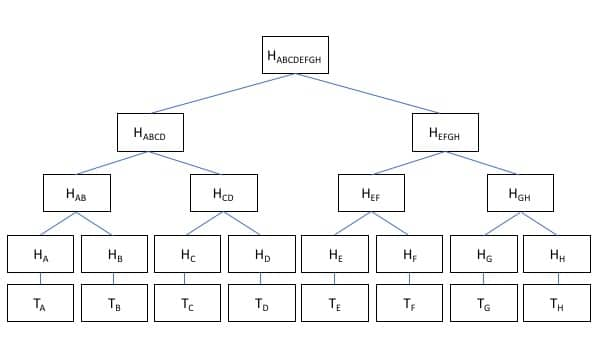
\includegraphics[width=\textwidth]{merkletree}
\end{frame}

\begin{frame}
  \frametitle{Block Header 4/4}
  \begin{itemize}
  \item Previous block hashes link blocks and transactions they contain into a
    linear sequence chain via a cryptographic commitments.
  \item Changing a single bit in a transaction completely changes the merkle
    root, which changes block hash, which, in turn changes hash of the next
    block and so on.
  \end{itemize}
  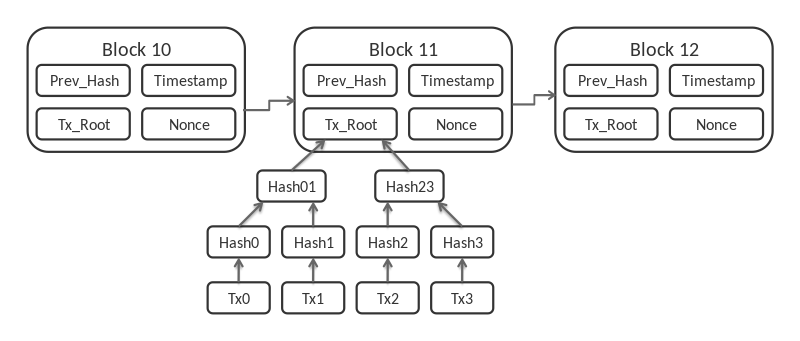
\includegraphics[width=\textwidth]{block-chain}
\end{frame}

\begin{frame}
  \frametitle{Mining}
  \begin{itemize}
  \item \textbf{Mining} is a process of computing Proof-of-Work solutions for
    new blocks.
  \item Miner
    \begin{itemize}
    \item selects a number of pending transactions,
    \item builds a Merkle tree and uses its root to construct the new block
      header with the last known block's hash as the previous block hash.
    \item performs a brute force search of the Proof-of-Work solution
      $$SHA256(SHA256(BlockHeader)) < Target$$
    \item if the PoW solution is found \textbf{before} an alternative solution
      is received over the peer-to-peer network, it can be published for the
      network to accept it as the new highest known block.
    \end{itemize}
  \end{itemize}
\end{frame}

\begin{frame}
  \frametitle{Coinbase Transaction and Halving Events}
  \begin{itemize}
  \item In order to incentivize miners to do their job, Bitcoin Protocol allows
    to add a special transaction at the beginning of the transaction list of
    each new block.
  \item This transaction is called \textbf{coinbase transaction} and has no
    inputs, only outputs, thus ``generating'' new bitcoins.
  \item Additionally, miners can add all transaction input-output amount
    differences (\textit{transaction fees}) to the coinbase transaction amount.
  \item \textbf{Halving events} - in order to keep bitcoin supply limited, the
    amount of new bitcoins started with 50 BTC and is reduced by the factor of 2
    every 210000 blocks, eventually reaching 0, at which point the bitcoin
    supply will stop growing.
  \end{itemize}
\end{frame}

\begin{frame}
  \frametitle{Useful Resources}
  \begin{itemize}
  \item Learn me a Bitcoin by Greg Walker - a great resource that explains
    multiple technical details about Bitcoin
    \begin{itemize}
    \item https://learnmeabitcoin.com/
    \end{itemize}
  \end{itemize}
\end{frame}

\begin{frame}
  \frametitle{The End}
  \begin{center}
    Thank you!
  \end{center}
\end{frame}

\end{document}

%%% Local Variables:
%%% mode: latex
%%% TeX-master: t
%%% End:
